\documentclass[professionalfonts]{beamer}
\newif\ifita
\itatrue % comment out to hide answers
\itafalse
\usepackage[familydefault,light]{Chivo} 
\usepackage[T1]{fontenc}
\usenavigationsymbolstemplate{}
\usepackage[]{hyperref}
\usepackage{tikz,pgf,pgfarrows,pgfnodes,pgfbaseimage}
\graphicspath{{./Pics/}}
\usetikzlibrary{shapes}
\usepackage{setspace}
\newcommand{\evi}[1]{{\colorbox{yellow!50}{{#1}}}}
\newcommand{\exe}[1]{{\color{black!50}{{#1}}}}
\newcommand{\kw}[1]{{\colorbox{black!30}{\color{white}{#1}}}}
\tikzstyle{nd}=[circle,draw=black,thick,minimum size=.8cm,inner sep=1pt]
\setbeamercovered{transparent}
\usetheme{Singapore}
\tikzstyle{nodo}=[ellipse,draw=black!60,fill=black!10,line width=.7pt,minimum width=.7cm,minimum height=.4cm]
\usecolortheme[named=gray]{structure}
\setbeamercolor{block title}{bg=black!20,fg=black}
\setbeamercolor{block body}{bg=black!10,fg=black}

\usepackage{comment}
%%%%%%%%%%%%%%%%%%%%%
\ifita
\title{Algoritmi Numerici (Parte IV)}
\subtitle{[Lezione 4] Numerical Integration}
\else
\title{Numerics (Part IV)}
\subtitle{[Lecture 4] Numerical Integration}
\fi
\date{}
\author{Alessandro Antonucci\\{\tt alessandro.antonucci@supsi.ch}}
%%%%%%%%%%%%%%%%%%%%%%%%%%%%
\begin{document}
\maketitle
\setbeamercovered{}
    %\setstretch{1.3}
%    \frame{\frametitle{\ifita Approccio Sp-line \else Sp-line Approach \fi}


%\documentclass[professionalfonts]{beamer}
%\usepackage[english]{babel}
%\usepackage{verbatim}
%\usepackage{graphicx}
%\usepackage{pgfplots}
%\usetikzlibrary{automata,topaths}
%\pgfplotsset{width=7cm,compat=1.8}
%\usepackage{pgfplotstable}
%\pgfmathsetseed{1138} % set the random seed
%\pgfplotstableset{ % Define the equations for x and y
%    create on use/x/.style={create col/expr={42+2*\pgfplotstablerow}},
%    create on use/y/.style={create col/expr={(0.6*\thisrow{x}+130)+5*rand}}
%}
% create a new table with 30 rows and columns x and y:
%\pgfplotstablenew[columns={x,y}]{30}\loadedtable

%\usepackage[familydefault,light]{Chivo} 
\usepackage[T1]{fontenc}
\usenavigationsymbolstemplate{}
\usepackage[]{hyperref}
\usepackage{tikz,pgf,pgfarrows,pgfnodes,pgfbaseimage}
\graphicspath{{./Pics/}}
\usetikzlibrary{shapes}
\usepackage{setspace}
\newcommand{\evi}[1]{{\colorbox{yellow!50}{{#1}}}}
\newcommand{\exe}[1]{{\color{black!50}{{#1}}}}
\newcommand{\kw}[1]{{\colorbox{black!30}{\color{white}{#1}}}}
\tikzstyle{nd}=[circle,draw=black,thick,minimum size=.8cm,inner sep=1pt]
\setbeamercovered{transparent}
\usetheme{Singapore}
\tikzstyle{nodo}=[ellipse,draw=black!60,fill=black!10,line width=.7pt,minimum width=.7cm,minimum height=.4cm]
\usecolortheme[named=gray]{structure}
\setbeamercolor{block title}{bg=black!20,fg=black}
\setbeamercolor{block body}{bg=black!10,fg=black}

%%%%%%%%%%%%%%%%%%%%%
%\title{Algoritmi Numerici (Parte IV)}
%\subtitle{Lezione 4: integrazione numerica}
%\author{Alessandro Antonucci\\{\tt alessandro.antonucci@supsi.ch}}
%\date{}
%%%%%%%%%%%%%%%%%%%%%%%%%%%%
%\begin{document}
%\maketitle
%\setbeamercovered{}
\frame{\frametitle{\ifita Integrazione Numerica \else Numerical Integration\fi}
\begin{itemize}
\ifita
\item Integrale definito di una funzione $\int_{a}^b f(x) \cdot \mathrm{d}x$?
\item Se conosco $F(x)$ tale che $F'(x)=\frac{\mathrm{d}f}{\mathrm{d}x}$
\item Allora $\int_{a}^b f(x) \mathrm{d}x=F(b)-F(a)$
\item Non tutte le funzioni sono integrabili in senso indefinito (es. $f(x)=e^{-x^2}$)
\item Idea: campionare $f$ in $n+1$ punti, interpolare e poi integrare la funzione interpolante
\item Banale con interpolazione mediante sp-line lineare
\else
\item Definite Integral of a function $\int_{a}^b f(x) \cdot \mathrm{d}x$?
\item Given $F(x)$ such that $F'(x)=\frac{\mathrm{d}f}{\mathrm{d}x}$
\item Then $\int_{a}^b f(x) \mathrm{d}x=F(b)-F(a)$
\item Not every function can be integrated (ex. $f(x)=e^{-x^2}$)
\item Idea: sampling $f$ in $n+1$ points, interpolating, and integrating the interpolating function
\item Trivial for interpolation based on linear sp-line
\fi
\end{itemize}}
\frame{\frametitle{\ifita Metodo dei trapezi \else Trapezoidal Rule \fi}
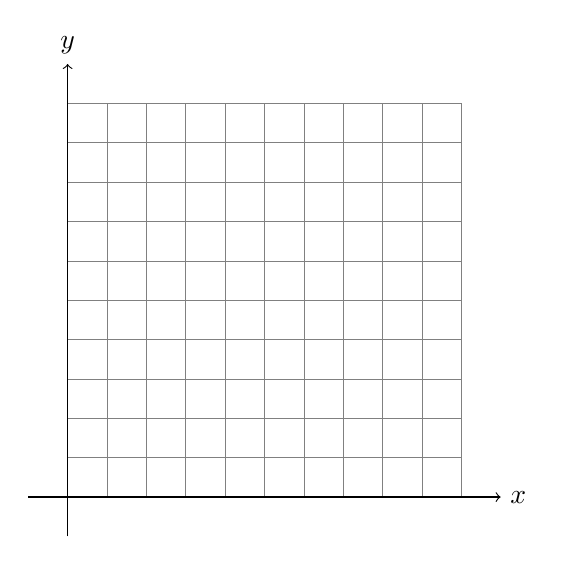
\begin{tikzpicture}[scale=5.0]
\draw[step=0.1,very thin,color=gray] (0.0,0.0) grid (1.0,1.0);
\draw[->] (-0.1,0) -- (1.1,0) node[right] {$x$};
\draw[->] (0,-0.1) -- (0,1.1) node[above] {$y$};
\draw[samples=400,domain=0:1,color=blue,thick] plot[id=exp] function{sqrt(1.0-x*x)};
\end{tikzpicture}}

\frame{\frametitle{\ifita Metodo dei trapezi \else Trapezoidal Rule \fi}
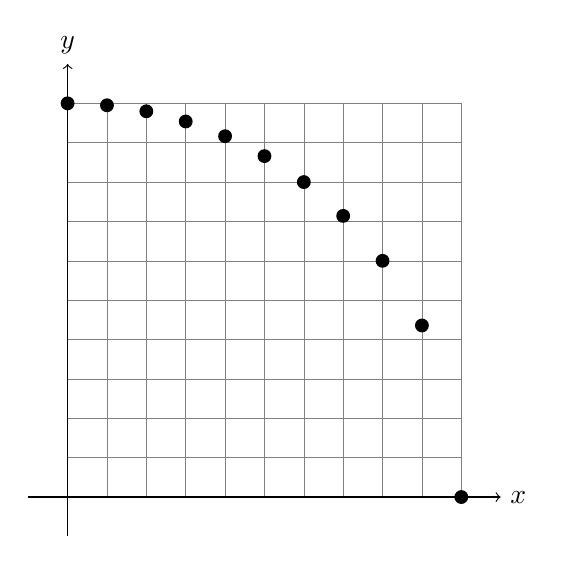
\begin{tikzpicture}[scale=5.0]
\draw[step=0.1,very thin,color=gray] (0.0,0.0) grid (1.0,1.0);
\draw[->] (-0.1,0) -- (1.1,0) node[right] {$x$};
\draw[->] (0,-0.1) -- (0,1.1) node[above] {$y$};
\draw[samples=400,domain=0:1,color=blue,thick] plot[id=exp] function{sqrt(1.0-x*x)};
\fill(0.0,1.0) circle[radius=.5pt,green];
\fill(0.1,0.995) circle[radius=.5pt,green];
\fill(0.2,0.9798) circle[radius=.5pt,green];
\fill(0.3,0.95393) circle[radius=.5pt,green];
\fill(0.4,0.9165) circle[radius=.5pt,green];
\fill(0.5,0.866) circle[radius=.5pt,green];
\fill(0.6,0.8) circle[radius=.5pt,green];
\fill(0.7,0.71414) circle[radius=.5pt,green];
\fill(0.8,0.6) circle[radius=.5pt,green];
\fill(0.9,0.4358) circle[radius=.5pt,green];
\fill(1.0,0) circle[radius=.5pt,green];
\end{tikzpicture}}

\frame{\frametitle{\ifita Metodo dei trapezi \else Trapezoidal Rule \fi}
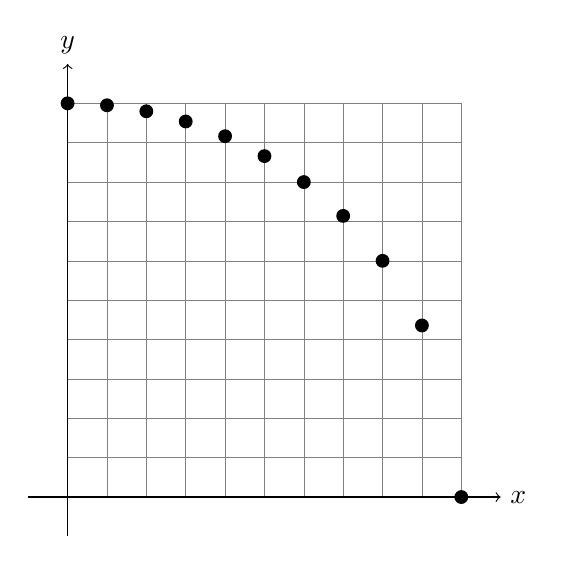
\begin{tikzpicture}[scale=5.0]
\draw[step=0.1,very thin,color=gray] (0.0,0.0) grid (1.0,1.0);
\draw[->] (-0.1,0) -- (1.1,0) node[right] {$x$};
\draw[->] (0,-0.1) -- (0,1.1) node[above] {$y$};
\fill(0.0,1.0) circle[radius=.5pt,green];
\fill(0.1,0.995) circle[radius=.5pt,green];
\fill(0.2,0.9798) circle[radius=.5pt,green];
\fill(0.3,0.95393) circle[radius=.5pt,green];
\fill(0.4,0.9165) circle[radius=.5pt,green];
\fill(0.5,0.866) circle[radius=.5pt,green];
\fill(0.6,0.8) circle[radius=.5pt,green];
\fill(0.7,0.71414) circle[radius=.5pt,green];
\fill(0.8,0.6) circle[radius=.5pt,green];
\fill(0.9,0.4358) circle[radius=.5pt,green];
\fill(1.0,0) circle[radius=.5pt,green];
\end{tikzpicture}}

\frame{\frametitle{\ifita Metodo dei trapezi \else Trapezoidal Rule \fi}
\begin{tikzpicture}[scale=5.0]
\draw[->] (-0.1,0) -- (1.1,0) node[right] {$x$};
\draw[->] (0,-0.1) -- (0,1.1) node[above] {$y$};
\fill(0.0,1.0) circle[radius=.5pt,green];
\fill(0.1,0.995) circle[radius=.5pt,green];
\fill(0.2,0.9798) circle[radius=.5pt,green];
\fill(0.3,0.95393) circle[radius=.5pt,green];
\fill(0.4,0.9165) circle[radius=.5pt,green];
\fill(0.5,0.866) circle[radius=.5pt,green];
\fill(0.6,0.8) circle[radius=.5pt,green];
\fill(0.7,0.71414) circle[radius=.5pt,green];
\fill(0.8,0.6) circle[radius=.5pt,green];
\fill(0.9,0.4358) circle[radius=.5pt,green];
\fill(1.0,0) circle[radius=.5pt,green];
\draw (0.0,1.0)--(0.1,0.995)--(0.2,0.9798)--(0.3,0.95393)--(0.4,0.9165)--(0.5,0.866)--(0.6,0.8)--(0.7,0.71414)--(0.8,0.6)--(0.9,0.4358)--(1.0,0);
\end{tikzpicture}}


\frame{\frametitle{\ifita Metodo dei trapezi \else Trapezoidal Rule \fi}
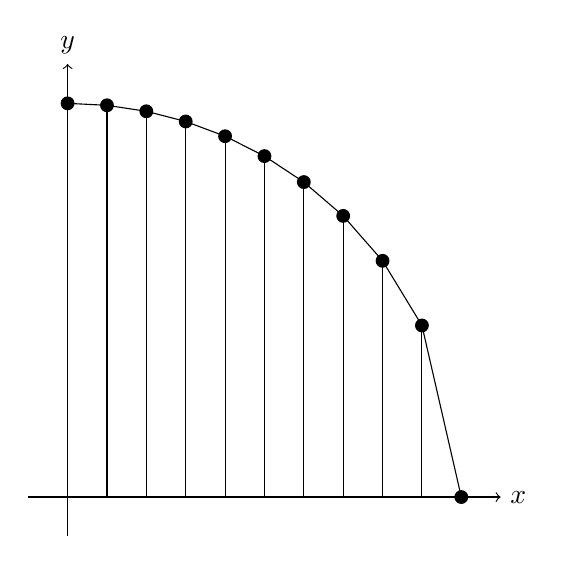
\begin{tikzpicture}[scale=5.0]
\draw[->] (-0.1,0) -- (1.1,0) node[right] {$x$};
\draw[->] (0,-0.1) -- (0,1.1) node[above] {$y$};
\fill(0.0,1.0) circle[radius=.5pt,green];
\fill(0.1,0.995) circle[radius=.5pt,green];
\fill(0.2,0.9798) circle[radius=.5pt,green];
\fill(0.3,0.95393) circle[radius=.5pt,green];
\fill(0.4,0.9165) circle[radius=.5pt,green];
\fill(0.5,0.866) circle[radius=.5pt,green];
\fill(0.6,0.8) circle[radius=.5pt,green];
\fill(0.7,0.71414) circle[radius=.5pt,green];
\fill(0.8,0.6) circle[radius=.5pt,green];
\fill(0.9,0.4358) circle[radius=.5pt,green];
\fill(1.0,0) circle[radius=.5pt,green];
\draw (0.0,1.0)--(0.1,0.995)--(0.2,0.9798)--(0.3,0.95393)--(0.4,0.9165)--(0.5,0.866)--(0.6,0.8)--(0.7,0.71414)--(0.8,0.6)--(0.9,0.4358)--(1.0,0);
\draw (0.1,0) -- (0.1,0.995);
\draw (0.2,0) -- (0.2,0.9798);
\draw (0.3,0) --(0.3,0.95393);
\draw (0.4,0) --(0.4,0.9165);
\draw (0.5,0) --(0.5,0.866);
\draw (0.6,0) --(0.6,0.8);
\draw (0.7,0) --(0.7,0.71414);
\draw (0.8,0) --(0.8,0.6);
\draw (0.9,0) --(0.9,0.4358);
\end{tikzpicture}}


\frame{\frametitle{\ifita Metodo dei trapezi \else Trapezoidal Rule \fi}
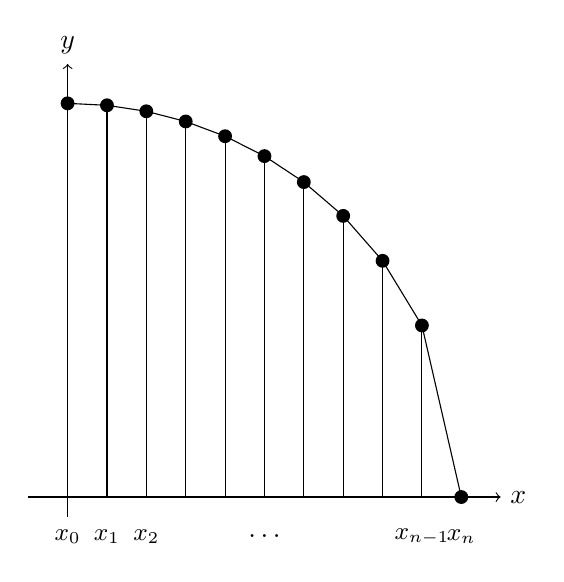
\begin{tikzpicture}[scale=5.0]
\draw[->] (-0.1,0) -- (1.1,0) node[right] {$x$};
\draw[->] (0,-0.05) -- (0,1.1) node[above] {$y$};
\fill(0.0,1.0) circle[radius=.5pt,green];
\fill(0.1,0.995) circle[radius=.5pt,green];
\fill(0.2,0.9798) circle[radius=.5pt,green];
\fill(0.3,0.95393) circle[radius=.5pt,green];
\fill(0.4,0.9165) circle[radius=.5pt,green];
\fill(0.5,0.866) circle[radius=.5pt,green];
\fill(0.6,0.8) circle[radius=.5pt,green];
\fill(0.7,0.71414) circle[radius=.5pt,green];
\fill(0.8,0.6) circle[radius=.5pt,green];
\fill(0.9,0.4358) circle[radius=.5pt,green];
\fill(1.0,0) circle[radius=.5pt,green];
\draw (0.0,1.0)--(0.1,0.995)--(0.2,0.9798)--(0.3,0.95393)--(0.4,0.9165)--(0.5,0.866)--(0.6,0.8)--(0.7,0.71414)--(0.8,0.6)--(0.9,0.4358)--(1.0,0);
\draw (0.1,0) -- (0.1,0.995);
\draw (0.2,0) -- (0.2,0.9798);
\draw (0.3,0) --(0.3,0.95393);
\draw (0.4,0) --(0.4,0.9165);
\draw (0.5,0) --(0.5,0.866);
\draw (0.6,0) --(0.6,0.8);
\draw (0.7,0) --(0.7,0.71414);
\draw (0.8,0) --(0.8,0.6);
\draw (0.9,0) --(0.9,0.4358);
\node (A) at (0.0,-0.1) {\small $x_0$};
\node (A) at (0.1,-0.1) {\small $x_1$};
\node (A) at (0.2,-0.1) {\small $x_2$};
\node (A) at (0.5,-0.1) {$\ldots$};
\node (A) at (0.9,-0.1) {\small $x_{n-1}$};
\node (A) at (1.0,-0.1) {\small $x_n$};
\end{tikzpicture}}


\frame{\frametitle{\ifita Metodo dei trapezi \else Trapezoidal Rule \fi}
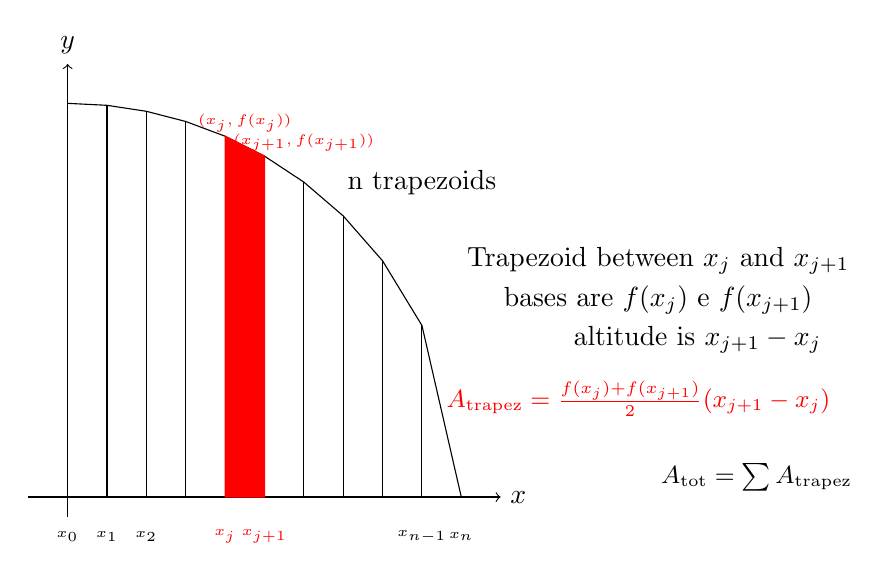
\begin{tikzpicture}[scale=5.0]
\draw[->] (-0.1,0) -- (1.1,0) node[right] {$x$};
\draw[->] (0,-0.05) -- (0,1.1) node[above] {$y$};
\draw (0.0,1.0)--(0.1,0.995)--(0.2,0.9798)--(0.3,0.95393)--(0.4,0.9165)--(0.5,0.866)--(0.6,0.8)--(0.7,0.71414)--(0.8,0.6)--(0.9,0.4358)--(1.0,0);
\draw (0.1,0) -- (0.1,0.995);
\draw (0.2,0) -- (0.2,0.9798);
\draw (0.3,0) --(0.3,0.95393);
\draw (0.4,0) --(0.4,0.9165);
\draw (0.5,0) --(0.5,0.866);
\draw (0.6,0) --(0.6,0.8);
\draw (0.7,0) --(0.7,0.71414);
\draw (0.8,0) --(0.8,0.6);
\draw (0.9,0) --(0.9,0.4358);
\node (A) at (0.0,-0.1) {\tiny $x_0$};
\node (A) at (0.1,-0.1) {\tiny $x_1$};
\node (A) at (0.2,-0.1) {\tiny $x_2$};
\node (A) at (0.9,-0.1) {\tiny $x_{n-1}$};
\node (A) at (1.0,-0.1) {\tiny $x_n$};
\node (A) at (0.9,0.8) {n \ifita trapezi \else trapezoids \fi};
\pause
\node (A) at (1.5,0.6) {\ifita Considero trapezio fra \else Trapezoid between \fi $x_j$ \ifita e \else and \fi $x_{j+1}$};
\draw[fill,red] (0.4,0.0) -- (0.5,0.0) -- (0.5,0.866) -- (0.4,0.9165) -- (0.4,0.0);
\node[color=red] (A) at (0.4,-0.1) {\tiny $x_{j}$};
\node[color=red] (A) at (0.5,-0.1) {\tiny $x_{j+1}$};
\pause
\node (A) at (1.5,0.5) {\ifita le sue basi sono \else bases are \fi $f(x_j)$ e $f(x_{j+1})$};
\node[color=red] (A) at (0.45,0.95) {\tiny $(x_j,f(x_{j}))$};
\node[color=red] (A) at (0.6,0.9) {\tiny $(x_{j+1},f(x_{j+1}))$};
\pause
\node (A) at (1.6,0.4) {\ifita la sua altezza \else altitude is \fi $x_{j+1}-x_j$};
\pause
\node (A) at (1.45,0.25) {\color{red}{\small $A_{\mathrm{trapez}} = \frac{f(x_j)+f(x_{j+1})}{2} (x_{j+1}-x_j)$}};
\pause
\node (A) at (1.75,0.05) {\small $A_{\mathrm{tot}} =\sum A_{\mathrm{trapez}}$};
\end{tikzpicture}}

\frame{
\centering
\Large
 $A_{\mathrm{tot}} = \sum_{j=0}^{n-1}  \frac{f(x_j)+f(x_{j+1})}{2} (x_{j+1}-x_j)$
\pause
\vskip 10mm
\ifita
Se le $x$ dei punti di appoggio sono equidistanti, i trapezi hanno tutti la stessa altezza
\else
If points are at same distance on the $x$-axis, all trapezoids have same altitude
\fi
 $\frac{x_n-x_0}{n}$
\vskip 10mm
\pause
 $A_{\mathrm{tot}} = \frac{x_n-x_0}{n} \sum_{j=0}^{n-1}  \frac{f(x_j)+f(x_{j+1})}{2}$
}


\frame{%\frametitle{Metodo dei trapezi}
\begin{columns}
\begin{column}{0.4\textwidth}
\begin{tikzpicture}[scale=5.0]
\draw[->] (-0.1,0) -- (1.1,0) node[right] {$x$};
\draw[->] (0,-0.1) -- (0,1.1) node[above] {$y$};
\draw (0.1,0.0)--(0.1,0.995);
\draw(0.2,0.0)--(0.2,0.9798);
\draw(0.3,0.0)--(0.3,0.95393); 
\draw(0.4,0.0)--(0.4,0.9165); 
\draw(0.5,0.0)--(0.5,0.866); 
\draw(0.6,0.0)--(0.6,0.8);
\draw(0.7,0.0)--(0.7,0.71414); 
\draw(0.8,0.0)--(0.8,0.6);
\draw(0.9,0)--(0.9,0.4358);
\draw (0.0,1.0)--(0.1,0.995)--(0.2,0.9798)--(0.3,0.95393)--(0.4,0.9165)--(0.5,0.866)--(0.6,0.8)--(0.7,0.71414)--(0.8,0.6)--(0.9,0.4358)--(1.0,0);
\end{tikzpicture}
\end{column}
\begin{column}{0.4\textwidth}
\begin{itemize}
\item \ifita Area di ogni trapezio? \else Trapezoid area? \fi
\item \ifita Altezza per base maggiore pi\`u base minore diviso due \else long basis plus short basis by altitude divided by two \fi
\item \small $\sum_{i} (x_{i+1}-x_i) \frac{f(x_i)+f(x_{i+1})}{2}$
\ifita
\item $x$ equidistanti? stessa altezza
\else
\item same distance $x$? same altitudes
\fi
\end{itemize}
\end{column}
\end{columns}
$$A = \frac{x_n-x_0}{n} \sum_{i=0}^{n-1} \frac{f(x_i)+f(x_{i+1})}{2}$$}
\frame{
$$A = \frac{1}{10} \left( 
\frac{\sqrt{1.00}+\sqrt{0.99}}{2}+
\frac{\sqrt{0.99}+\sqrt{0.96}}{2}+ \right.$$
$$
\frac{\sqrt{0.96}+\sqrt{0.91}}{2}+
\frac{\sqrt{0.91}+\sqrt{0.84}}{2}+$$
$$\frac{\sqrt{0.84}+\sqrt{0.75}}{2}+
\frac{\sqrt{0.75}+\sqrt{0.64}}{2}+$$
$$\frac{\sqrt{0.64}+\sqrt{0.51}}{2}+
\frac{\sqrt{0.51}+\sqrt{0.36}}{2}+$$
$$\left.\frac{\sqrt{0.36}+\sqrt{0.19}}{2}+
\frac{\sqrt{0.19}+\sqrt{0.00}}{2}\right)\simeq 0.7761$$
$$\frac{\pi}{4} \simeq 0.7854$$ }
\end{document}
